\renewcommand{\theequation}{\theenumi}
\begin{enumerate}[label=\arabic*.,ref=\thesubsection.\theenumi]
\numberwithin{equation}{enumi}

\item
	\label{convex_code}
Find
\begin{align}
\label{eq2_1_circ}
	\min_{\mbf{x}}f\brak{\mbf{x}} = \norm{\vec{x}-\myvec{8\\6}}^2 = r^2 \\
\text{s.t.} \quad 	g\brak{\mbf{x}} = \myvec{1 & 1}\vec{x} - 9 = 0\label{eq2_1_line}
%	\quad g\brak{\mbf{x}} = x_1 + x_2 - 9 = 0
\end{align}
by plotting the circles $f\brak{\vec{x}}$
%
%\begin{equation}
% \norm{\vec{x}-\myvec{8\\6}}^2 =r^2
%%(x_1-8)^2 + (x_2-6)^2 = r^2
%\end{equation}
%
% $\mbf{x}= \myvec{x_1\\x_2}$, 
for different values of $r$ along with the line $g\brak{\mbf{x}}$.
%
%\begin{equation}
%\label{eq2_1_line}
%g\brak{\mbf{x}} = \myvec{1 & 1}\vec{x} - 9 = 0
%\end{equation} 
%
\\
\solution 
The following code plots Fig. \ref{fig.2.1}	

%	
\begin{lstlisting}
codes/optimization/2.1.py
\end{lstlisting}

%
\begin{figure}[!ht]
\centering
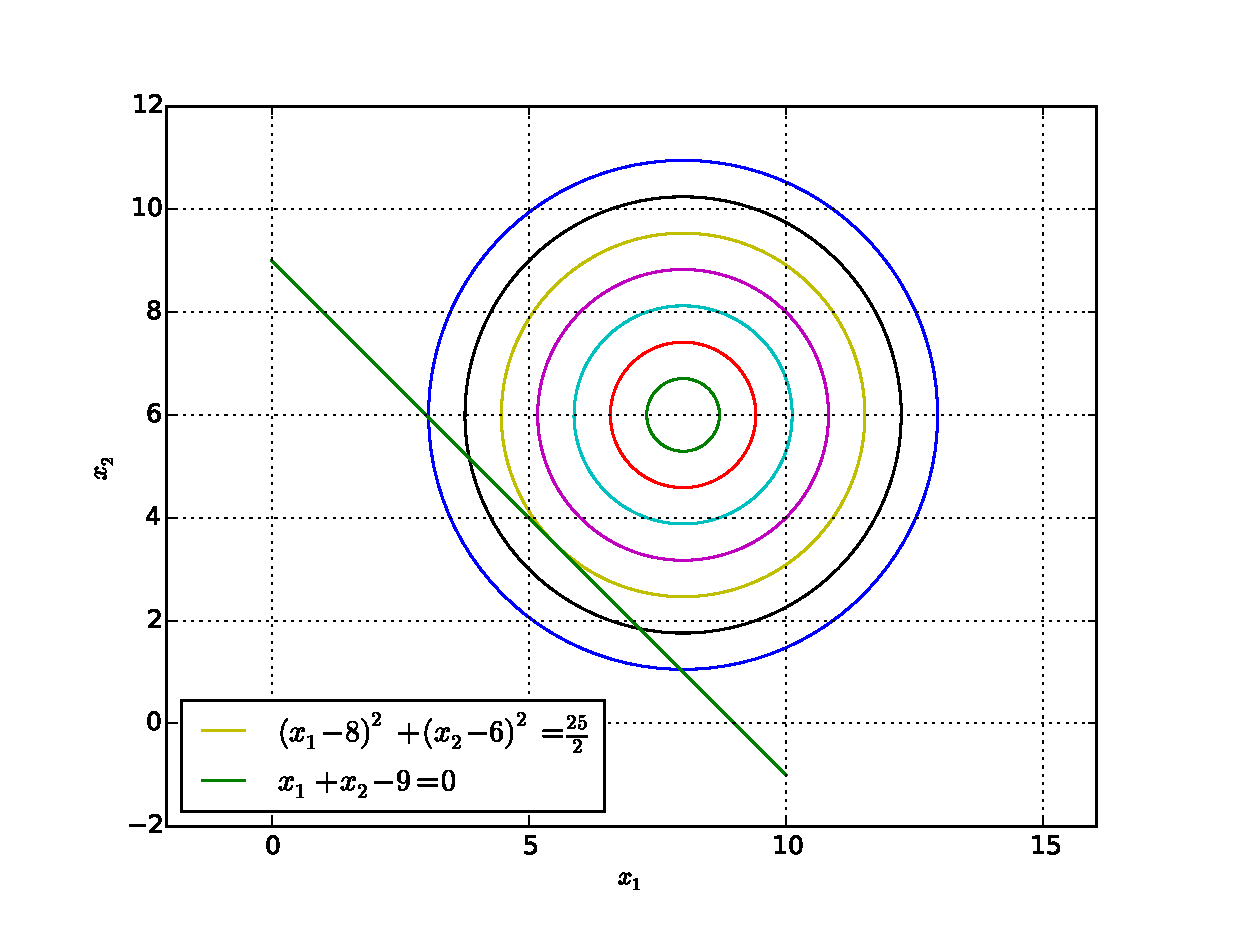
\includegraphics[width=\columnwidth]{./optimization/figs/2.1.eps}
\caption{ Finding $ \displaystyle \min_{\mbf{x}}f\brak{\mbf{x}}$}.
\label{fig.2.1}	
\end{figure}
%
\item Show that 
\begin{align}
\min r = \frac{5}{\sqrt{2}}
\end{align}
%Obtain a theoretical solution for problem \ref{convex_code} 
%%using coordinate geometry.
%
%\solution 
%From \eqref{eq2_1_line} and \eqref{eq2_1_circ}, 
%%
%\begin{align}
%r^2 & = (x_1-8)^2 + (3- x_1)^2 \\
%&= 2 x_1^2 - 22 x_1 + 73 \\
%\Rightarrow r^2 &= \frac{\brak{2x_1-11}^2 + 5^2}{2}
%\end{align}
%%
%which is minium when $x_1 = \frac{11}{2}, x_2 = \frac{7}{2}$.  The minimum value is $\frac{25}{2}$ and 
%the radius $r = \frac{5}{\sqrt{2}}$.
\item Show that 
\begin{align}
\nabla g(\vec{x}) = \myvec{1 \\ 1}
\end{align}
where
\begin{equation}
\nabla =  
\begin{pmatrix}
\frac{\partial}{\partial x_1} \\
\frac{\partial}{\partial x_2} 
\end{pmatrix}
\end{equation}

\item Show that 
\begin{align}
\nabla f(\vec{x}) = 2\cbrak{\vec{x}-\myvec{8 \\ 6}}
\end{align}
%
is the direction vector of the normal at $\vec{x}$.
\item From Fig. \ref{fig.2.1}, show that 
\begin{align}
\label{eq:opt_normal}
\nabla f(\vec{p}) = \lambda \nabla g(\vec{p}),
\end{align}
%
where $\vec{p}$ is the point of contact.
\item Use \eqref{eq:opt_normal} and $\vec{g(p)}=0$ from \eqref{eq2_1_line} to obtain $\vec{p}$.
\item
\label{lagrange}
	Define 
	\begin{equation}
	\label{lagrangian}
	L\brak{\mbf{x},\lambda} = f\brak{\mbf{x}} - \lambda g\brak{\mbf{x}}%, \quad \lambda > 0
	\end{equation}
and show that $\vec{p}$ can also be obtained by 
solving the equations
%
\begin{align}
\nabla L\brak{\mbf{x},\lambda} &= 0.
\label{tangent}
\end{align}
%
What is the sign of $\lambda$?  $L$ is known as the Lagrangian and the above technique is known as the Method of Lagrange Multipliers.

\solution
%From \eqref{eq2_1_line} and \eqref{eq2_1_circ}, 
%%
%\begin{align}
%L\brak{\mbf{x},\lambda} &= (x_1-8)^2 + (x_2-6)^2 - \lambda \brak{x_1 + x_2 - 9} \\
%\Rightarrow \nabla L\brak{\mbf{x},\lambda}  & = 
%\begin{pmatrix}
%2x_1  - 16 - \lambda \\
%2x_2 - 12 - \lambda \\
%x_1 + x_2 -9
%\end{pmatrix}
%\\
%&=
%\begin{pmatrix}
%2 &0 & - 1 \\
%0 &2 & - 1 \\
%1 & 1 & 0 
%\end{pmatrix}
%\begin{pmatrix}
%x_1 \\
%x_2 \\
%\lambda
%\end{pmatrix}
%= 
%\begin{pmatrix}
%16 \\
% 12 \\
%9
%\end{pmatrix}
%=
%0 
%\\
%\Rightarrow 
%\begin{pmatrix}
%x_1 \\
%x_2 \\
%\lambda
%\end{pmatrix}
%&= 
%\begin{pmatrix}
%\frac{11}{2} \\
% \frac{7}{2} \\
%-5
%\end{pmatrix}
%\end{align}
%%
%using the following python script.  Note that this method yields the same result as the previous exercises.  Thus, $\lambda$ is negative.
%	
\begin{lstlisting}
codes/optimization/2.3.py
\end{lstlisting}
\end{enumerate}
